\chapter{Methodology}
\vspace{-1.4em}
\begin{comment}
Note that methodology varies according to project type. Consider the engineering
tools you've learned throughout your degree in ANU to generate your results ---
this may also include the systems engineering approach.
\end{comment}

\section{Aircraft Dynamical Model}
\begin{figure}[htbp]
  \centering
  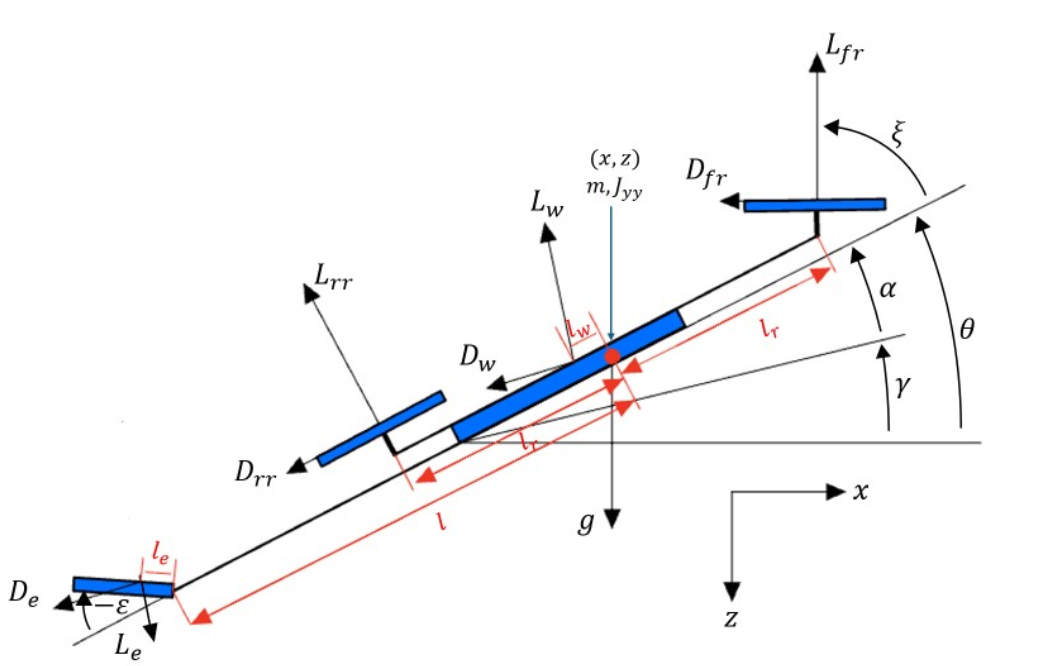
\includegraphics[width=0.8\textwidth]{images/model}
  \caption{Dynamical Model Diagram}
  \label{fig:model_diagram}
\end{figure}

\begin{comment}
The model used in this project is the same as that presented in Fraser Miller's Thesis, However some errors have been remedied and the aerodynamic coefficients have been re estimated to match real world flight logs of the Griffin Pro more closely. The new set of coefficients can be found in appendix X.
\end{comment}

The Model used in this project is based of that presented in Miller's thesis \cite{miller2025thesis}. As such the modeonly captures the longitundinal dynamics of the aircraft, this simplification was made as all of the behaviours being optimised are only present in the longitundinal case, while the lateral is being stabilised to trim level flight. 
The simplification to a two dimentional model means that the state space $X$ can be simlified from $\mathbb{R}^{12}$ to $\mathbb{R}^{6}$, the input space($U$) can also be simplified resulting in the spaces shown in \eqref{eq:state_input}

\begin{equation}
X=\begin{bmatrix} x&z&\theta&\dot{x}&\dot{z}&\dot{\theta}\end{bmatrix}^T, \qquad
U=\begin{bmatrix} \omega_{f}&\omega_{r}&\xi&\epsilon\end{bmatrix}^T
\label{eq:state_input}
\end{equation}

where
\begin{table}[ht]
  \centering

  \label{tab:basic_table}
  \begin{tabular}{|l|c|l|c|}
    \hline
    State &   & Input&   \\
    \hline
    $x$ & $e_{1}$ position (m)& $\omega_{f}$ & front rotor speed (rpm)\\
    $z$ & $e_{2}$ position (m)& $\omega_{r}$ & rear rotor speed (rpm)\\
    $\theta$ & pitch (rad)& $\xi$& front rotor tilt (rad)\\
    $\dot{x}$ & $e_{1}$ velocity (m/s)&$\epsilon$& elevator deflection (rad)\\
    $\dot{z}$ & $e_{2}$ velocity (m/s)&  & \\
    $\dot{\theta}$ & pitch rate (rad/s)& & \\
    \hline
  \end{tabular}
  \caption{Model States and Inputs}
\end{table}
\FloatBarrier


The dynamics of the system are shown in \eqref{eq:pos_dynamics} \& \eqref{eq:rot_dynamics}, which are an application of Newton's second law of motion rearranged.

\begin{equation}
\begin{bmatrix} \ddot{x}\\\ddot{z} \end{bmatrix}=\frac{1}{m}(R(\theta-\alpha)(F_{w}+F_{e})) + R(\theta+\xi)F_{fr}+R(\theta)F_{rr}+mg)
\label{eq:pos_dynamics}
\end{equation}
\begin{equation}
\ddot{\theta}=\frac{1}{J_{yy}}(    l_{w}R(-\alpha)  + F_{w_{\perp}}  + (lcos(\epsilon)+l_{e})R(-\alpha)F_{e_{\perp}}  - l_{r}R(\theta+\xi)F_{fr_{\perp}}  + l_{r}R(\theta)F_{rr_{\perp}}   )
\label{eq:rot_dynamics}
\end{equation}

where $R(\theta)$ is the standard two dimentaional rotation matrix.
\begin{comment} = \begin{bmatrix} cos(\theta) &-sin(\theta) \\sin(\theta) &cos(\theta) \end{bmatrix}$
\end{comment}

\subsection{Aerodynamic Surface Forces}
The aerodynamic surface (wing \& elevator) forces are modelled using a blended coefficents model to describe post-stall behaviour, as the standard approach of a linear model would mislead the trajectory optimisation when the aircraft would be in stall. The blended model approach utilises the standard linear airfoil coeffcient at angles of attack less than stall and smoothly transitions to a flat-plate model post-stall via a sigmoid function. 
\begin{equation}
L_{x}=\frac{1}{2} s_{x} \rho |v_{x}^{2}| C_{l_{x}}(\alpha_{x}), \quad D_{x}=\frac{1}{2} s_{x} \rho |v_{x}^{2}| C_{d_{x}}(\alpha_{x})
\label{eq:lift_drag}
\end{equation}
In the following set of equations (\eqref{eq:lift_drag}- \eqref{eq:simga}) $x$ represents a specfic aerodynamic surface of the aircraft. The total coeffcients \eqref{eq:coef} show how this blending occours.
\begin{equation}
\begin{split}
C_{l_{x}}(\alpha_{x}) = (1-\sigma_x)C_{l_{x_{airfroil}}}(\alpha_{x}) + \sigma_x C_{l_{{flatplate}}}(\alpha_{x}) \\
C_{d_{x}}(\alpha_{x}) = (1-\sigma_x)C_{d_{x_{airfroil}}}(\alpha_{x}) + \sigma_x C_{d_{{flatplate}}}(\alpha_{x})
\end{split}
\label{eq:coef}
\end{equation}

\begin{equation}
\begin{split}
C_{l_{x_{airfroil}}}(\alpha_{x})  = C_{l0_{x}} + C_{l\alpha_{x}}(\alpha_{x}), \quad C_{d_{x_{airfroil}}}(\alpha_{x})  = C_{d0} + C_{d\alpha_{x}}(\alpha_{x}^{2}), \\
\end{split}
\label{eq:coef2}
\end{equation}
\begin{equation}
C_{l_{{flatplate}}}(\alpha)  =2sin(\alpha)cos(\alpha), \quad C_{d_{{flatplate}}}(\alpha)  = 2sin^{2}(\alpha)
\label{eq:fp}
\end{equation}
This model for the elevator accounts for the variation in force due to the elevator deflection by applying a modifier to the elevator angle of attack proportional to the deflection. The value of this proportional gain ($\tau$) was fit log data from real world griffon pro flights.
\begin{equation}
\alpha_{w}= tan^{-1}\frac{\dot{z}}{\dot{x}} \qquad \alpha_{e} = \alpha_{w}+\epsilon\tau
\label{eq:aoas}
\end{equation}

\begin{equation}
\sigma_{x}(\alpha) = \frac{1+e^{-M_x(\alpha-t_{l_{x}})} + e^{M_x(\alpha-t_{u_{x}})}} {(1+e^{-M_x(\alpha-t_{l_{x}})})(1+e^{M_x(\alpha-t_{u_{x}})})}
\label{eq:simga}
\end{equation}

The Resulting Coeffcients of the wing can be seen in Figure \ref{fig:wing} where we have a continous function throughout $[-\pi,\pi]$


\begin{figure}[htbp]
  \centering
  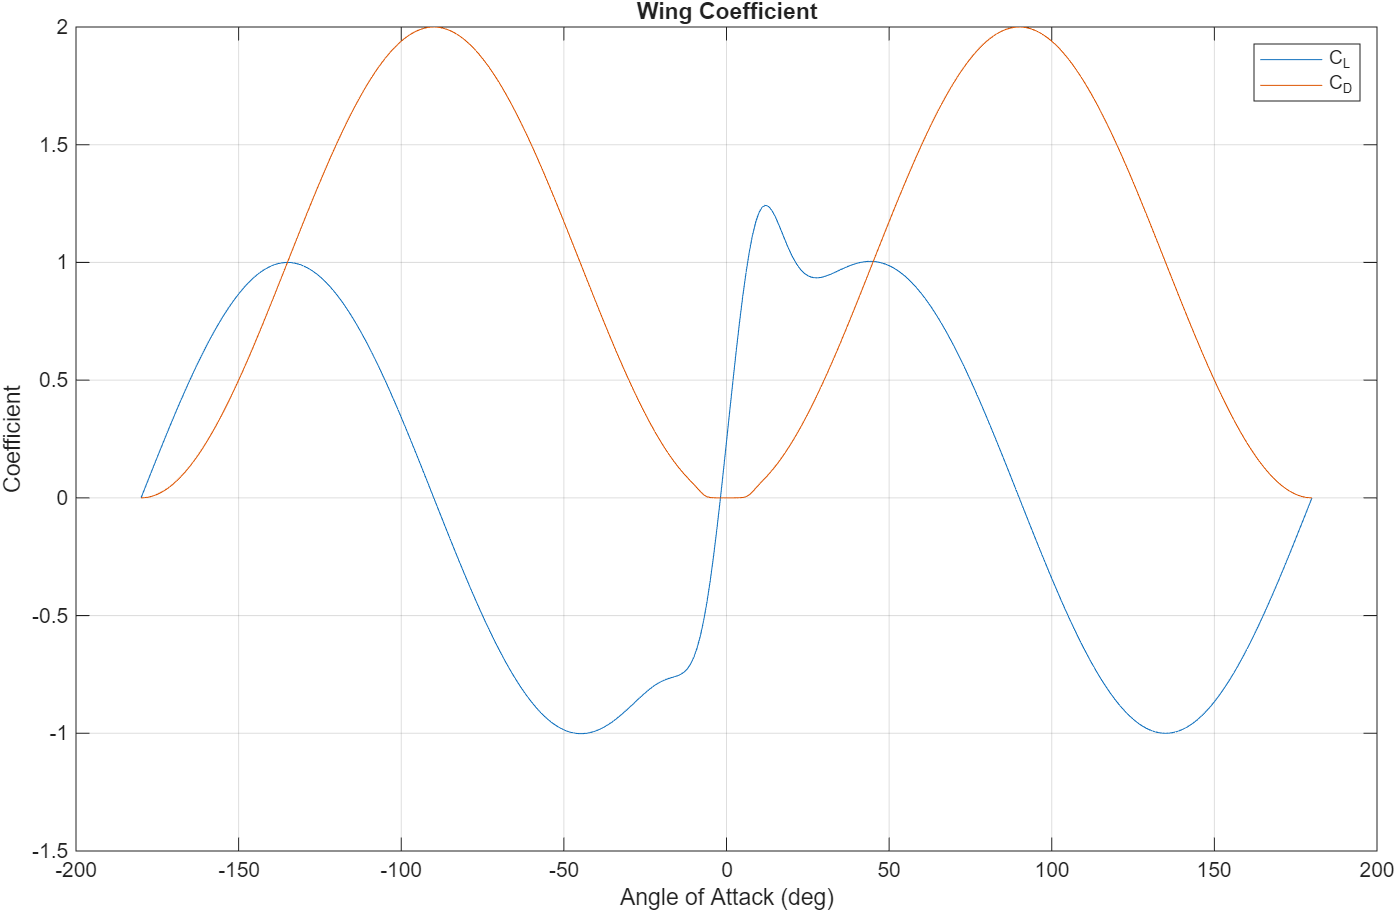
\includegraphics[width=0.8\textwidth]{images/Coefficient}
  \caption{Griffon Pro Wing Aerodynamic Coeffcients}
  \label{fig:wing}
\end{figure}

\begin{figure}[htbp]
  \centering
  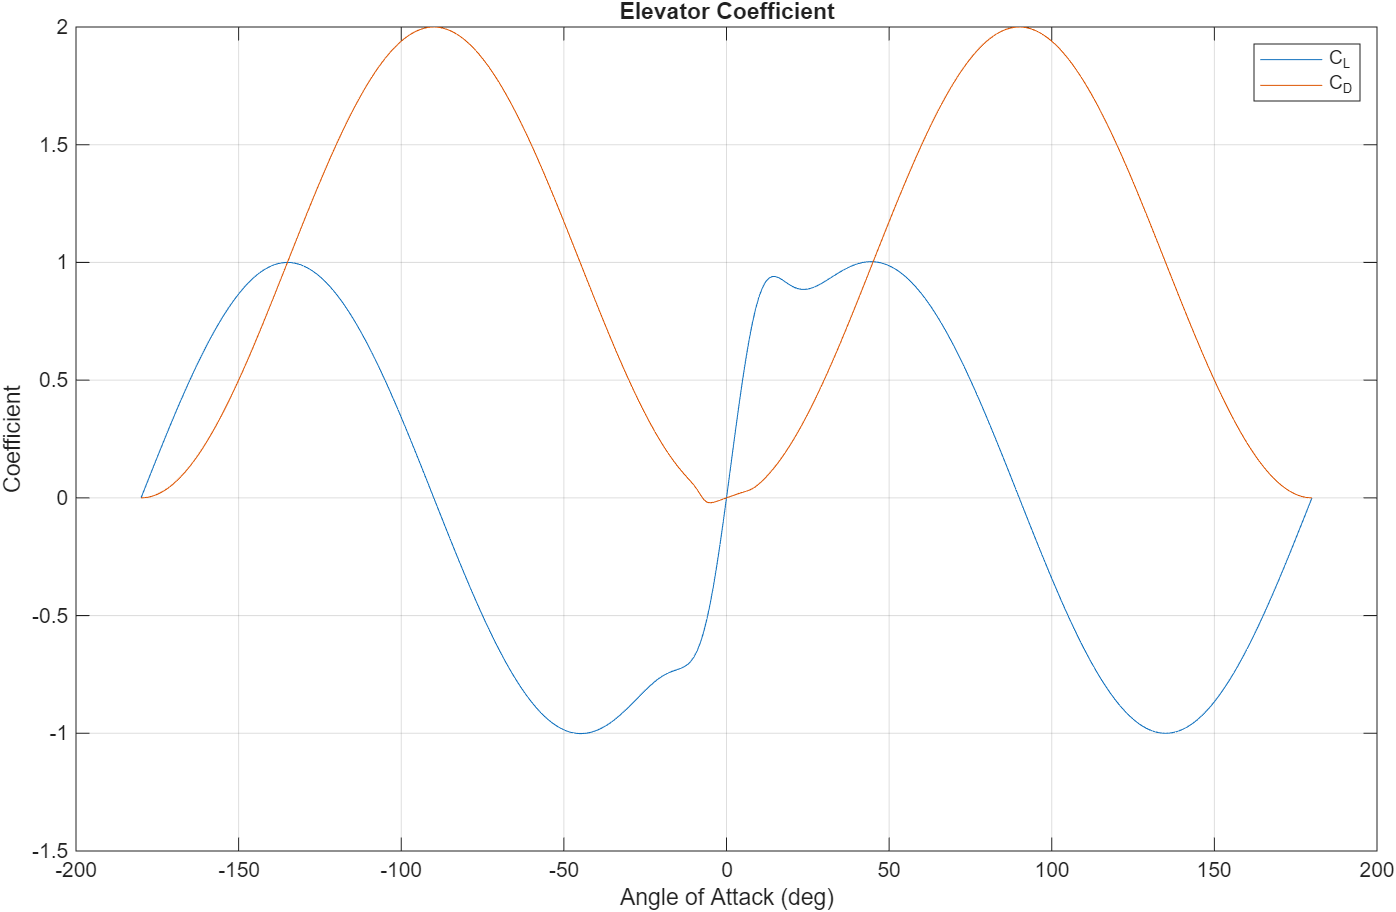
\includegraphics[width=0.8\textwidth]{images/Coefficient_elev}
  \caption{Griffon Pro Elevator Aerodynamic Coeffcients at $\epsilon=0$}
  \label{fig:elev}
\end{figure}

\FloatBarrier

\begin{table}[ht]
  \centering

  \label{tab:basic_table}
  \begin{tabular}{|l|c|l|c|}
    \hline
    Coeffcient & Value & Coeffcient & Value  \\
    \hline
    $C_{l0_{w}}$ & 1.9164 & $C_{l\alpha_{w}}$ & 11.6632\\
    $C_{l0_{e}}$ & 0 & $C_{l\alpha_{e}}$ & 6.8755\\
    $C_{d0_{w}}$ & 0.075 & $C_{d\alpha_{w}}$ & 4.015\\
    $C_{d0_{e}}$ & 0 .01& $C_{d\alpha_{e}}$ & 1.7968\\
    $t_{l_{w}}$ & -0.18 & $t_{u_{w}}$ & 0.28 \\
    $t_{l_{e}}$ & -0.28 & $t_{u_{e}}$ & 0.28 \\
    $M_w$ & 1 & $M_e$ & 26 \\
    $\tau$ & 2.7& & \\
   
    \hline
  \end{tabular}
  \caption{Aerodynamics Coefficients}
\end{table}
\FloatBarrier

\subsection{Rotor Forces}
The trajectory in section 3.2.6 utilises the non axial drag component the rotors produce when the freestream velocity has a perpendicular compenent to the rotor axle to dissipate kinetic energy from the aircraft, to model this behaviour the following equations were employed.


\begin{equation}
L_{front}=\frac{1}{2} N_{b} \rho c R_{r}^{3}\omega_{front}^{2} C_{T}, \qquad D_{front}=\frac{L_{front}(\dot{x}_{front})}{R_{r}\omega_{front}}
\label{eq:front_rotor}
\end{equation}
\begin{equation}
L_{rear}=\frac{1}{2} N_{b} \rho c R_{r}^{3} \omega_{rear}^{2} C_{T}, \qquad D_{rear}=\frac{L_{rear}(\dot{x}_{rear})}{R_{r}\omega_{rear}}
\label{eq:rear_rotor}
\end{equation}

where $N_{b}$ is the number of blades of the rotor, $\rho$ is air density,$c$ is the average chord of the airfoil, $R_{r}$ is the radius of the rotor and $C_{T}$ is the coefficient of thrust, it was estimated for hover by solving equation \eqref{eq:thrust_coeff} which is the lift of the front and rear rotors equated to the weight force of the aircraft with the values from a real world flight log substituted for $m,\rho,\omega$

\begin{equation}
\dot{X}_{front}=R_{IR}(\theta+\xi)X_{inertial}, \qquad \dot{X}_{rear}=R_{IR}(\theta+\xi)X_{inertial}, \qquad  {X}=\begin{bmatrix}{x}\\{z} \end{bmatrix}
\label{eq:rotor_velocity_sim}
\end{equation}

\begin{equation}
C_{T}=\frac{2mg}{N_{b} \rho c R_{r}^{3} (\omega_{front}+\omega_{rear})}
\label{eq:thrust_coeff}
\end{equation}






\begin{comment}
\subsection{Aerodynamic Surfaces}
\subsection{Rotor Forces}
\subsection{Dynamics}
\end{comment}
\section{Trajectory Optimisation}
The MATLAB library OptimTraj \cite{kelly2022optimtraj} was used to solve the optimisation problem for the transition trajectory. OptimTraj utilises MATLAB's fmincon solver.


\subsection{Constraints}
The constraints for the trajectory optimisation were as follows.
\begin{equation}
Y_{initial}=\begin{bmatrix}-400 &-50&-0.0623&22&0&0\end{bmatrix}^T
, \qquad
Y_{final}=\begin{bmatrix}0 &-10&0&0&0&0\end{bmatrix}^T
\label{eq:boundary_conditions}
\end{equation}
\begin{equation}
Y_{lower}=\begin{bmatrix} -\infty&-\infty&-\pi/10&-\infty&\infty&-\pi/12\end{bmatrix}^T
, \qquad
Y_{upper}=\begin{bmatrix} \infty&-10&\pi/3&22&\infty&\pi/12\end{bmatrix}^T
\label{eq:state_bounds}
\end{equation}
\begin{equation}
U_{lower}=\begin{bmatrix} 0&0&0&-\pi/4.75\end{bmatrix}^T
,\qquad
U_{upper}=\begin{bmatrix} 8500&8500&\pi/2&\pi/4.75\end{bmatrix}^T
\label{eq:input_bounds}
\end{equation}
\begin{equation}
11\pi/90-\alpha>=0,\qquad \alpha-\pi/18>=0
\label{eq:aoa_constraint}
\end{equation}
The control constraints are determined by the capabilities of the aircraft, with the exception of the tilt angle ($\xi$) a 15\% reduction to the upper limit was applied to ensure there was adequate control margin. $Y_{final}$ is set to a stationary hover 10m above the ground as to allow the stock ArduPilot to take over for the touch down and complete its disarming protocols uninterrupted, this height can also be altered along the state upper constraint for altitude to set a minimum height that the pilot feels is appropriate.
The final constraint was applied to the angle of attack of the airframe, to limit aggressiveness of the stalls the aircraft could perform, this too can be configured to a value the pilot deems appropriate.
\subsection{Initialisation}
The initialisation point of the optimisation was a straight line trajectory with the inputs at zero for all time.
\begin{equation}
Y_{initialisation}=\begin{bmatrix}Y_{initial},&Y_{final}\end{bmatrix},U_{initialisation}=0^{\mathbb{R}^{4 \times 2}}
\label{eq:initialisation}
\end{equation}
\subsection{Mesh Refinement}
The optimisation mesh would initially be calculated with 0.5s timesteps ($\Delta t$), and time would be a free variable. After the initial solution had converged, the total time would be rounded to the nearest 0.5s and be set as a constraint and the timesteps would be reduced to 0.25s, with the initial solution replacing the previous initialisations for state and control input. This process was repeated until a time step of 0.1s was achieved.
\subsection{Cost Function}
The goal of this optimisation is to find the most energy efficient landing transition trajectory, as such the cost function was set to the total energy consumed during the transition phase, with the assumption that elevator and tilt inputs would cause marginal differences the cost function was therefore simplified to be the energy the rotors require throughout the trajectory.

\begin{equation}
J_{trajectory} = \sum_{i=0}^{\frac{t_{f}}{\Delta t}} 2(P_{front_{i}} +P_{rear_{i}})\Delta t
\label{eq:traj_cost}
\end{equation}

The power estimates show in \ref{eq:traj_cost} are derived using the method shown in  \cite{miller2025thesis}, and can also be found in Appendix ??.

\subsection{Solution}
\begin{figure}[htbp]
  \centering
  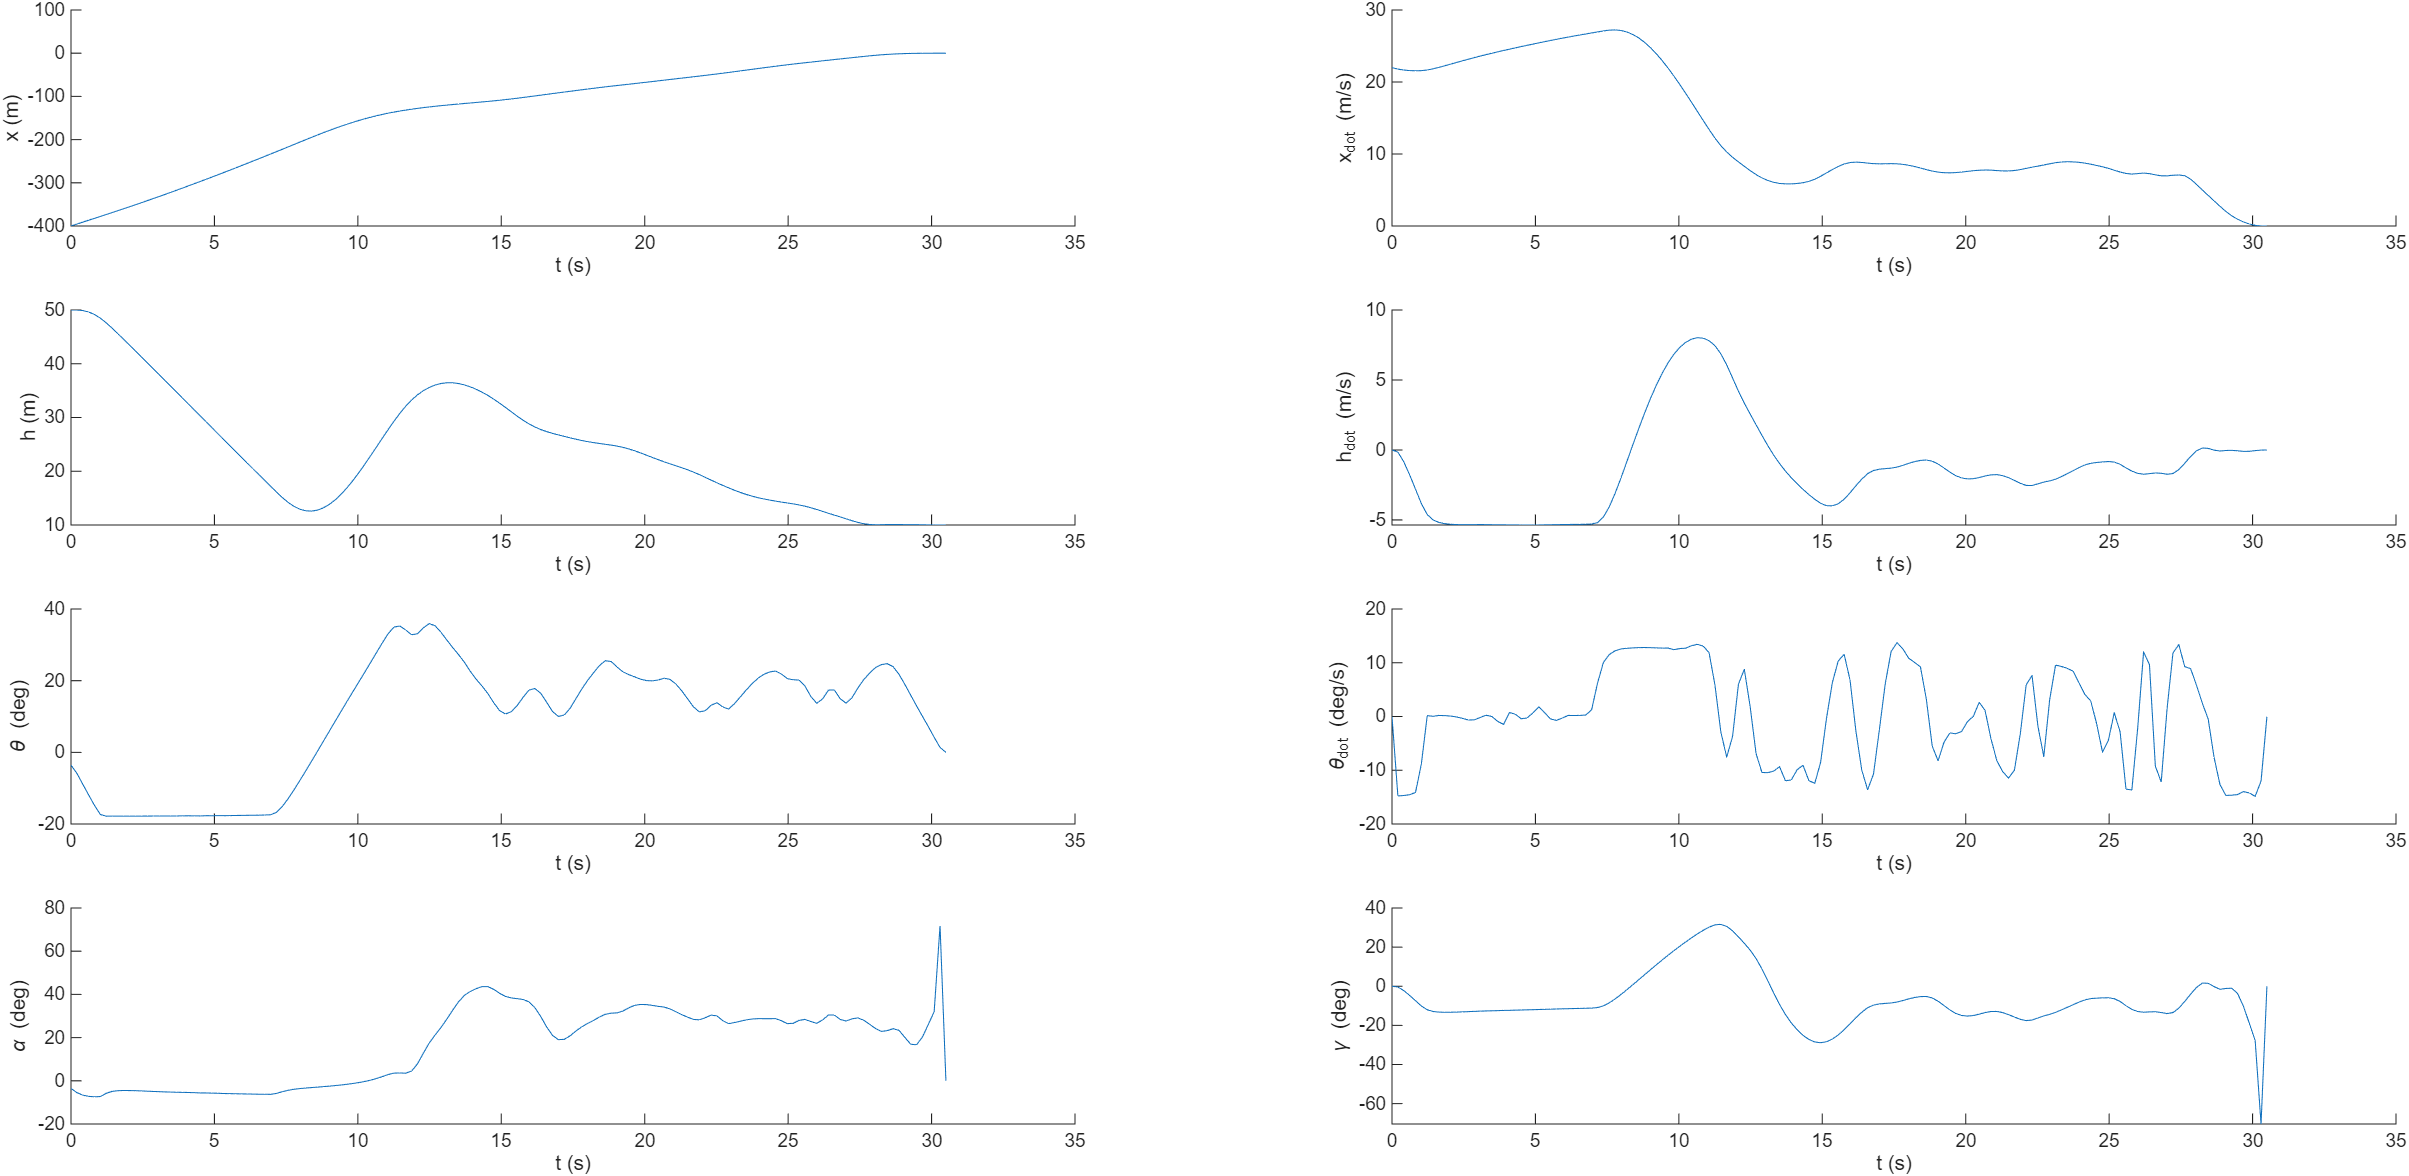
\includegraphics[width=0.8\textwidth]{images/open_loop_states}
  \caption{Trajectory Optimisation Solution States}
  \label{fig:Open-Loop States}
\end{figure}
\begin{figure}[htbp]
  \centering
  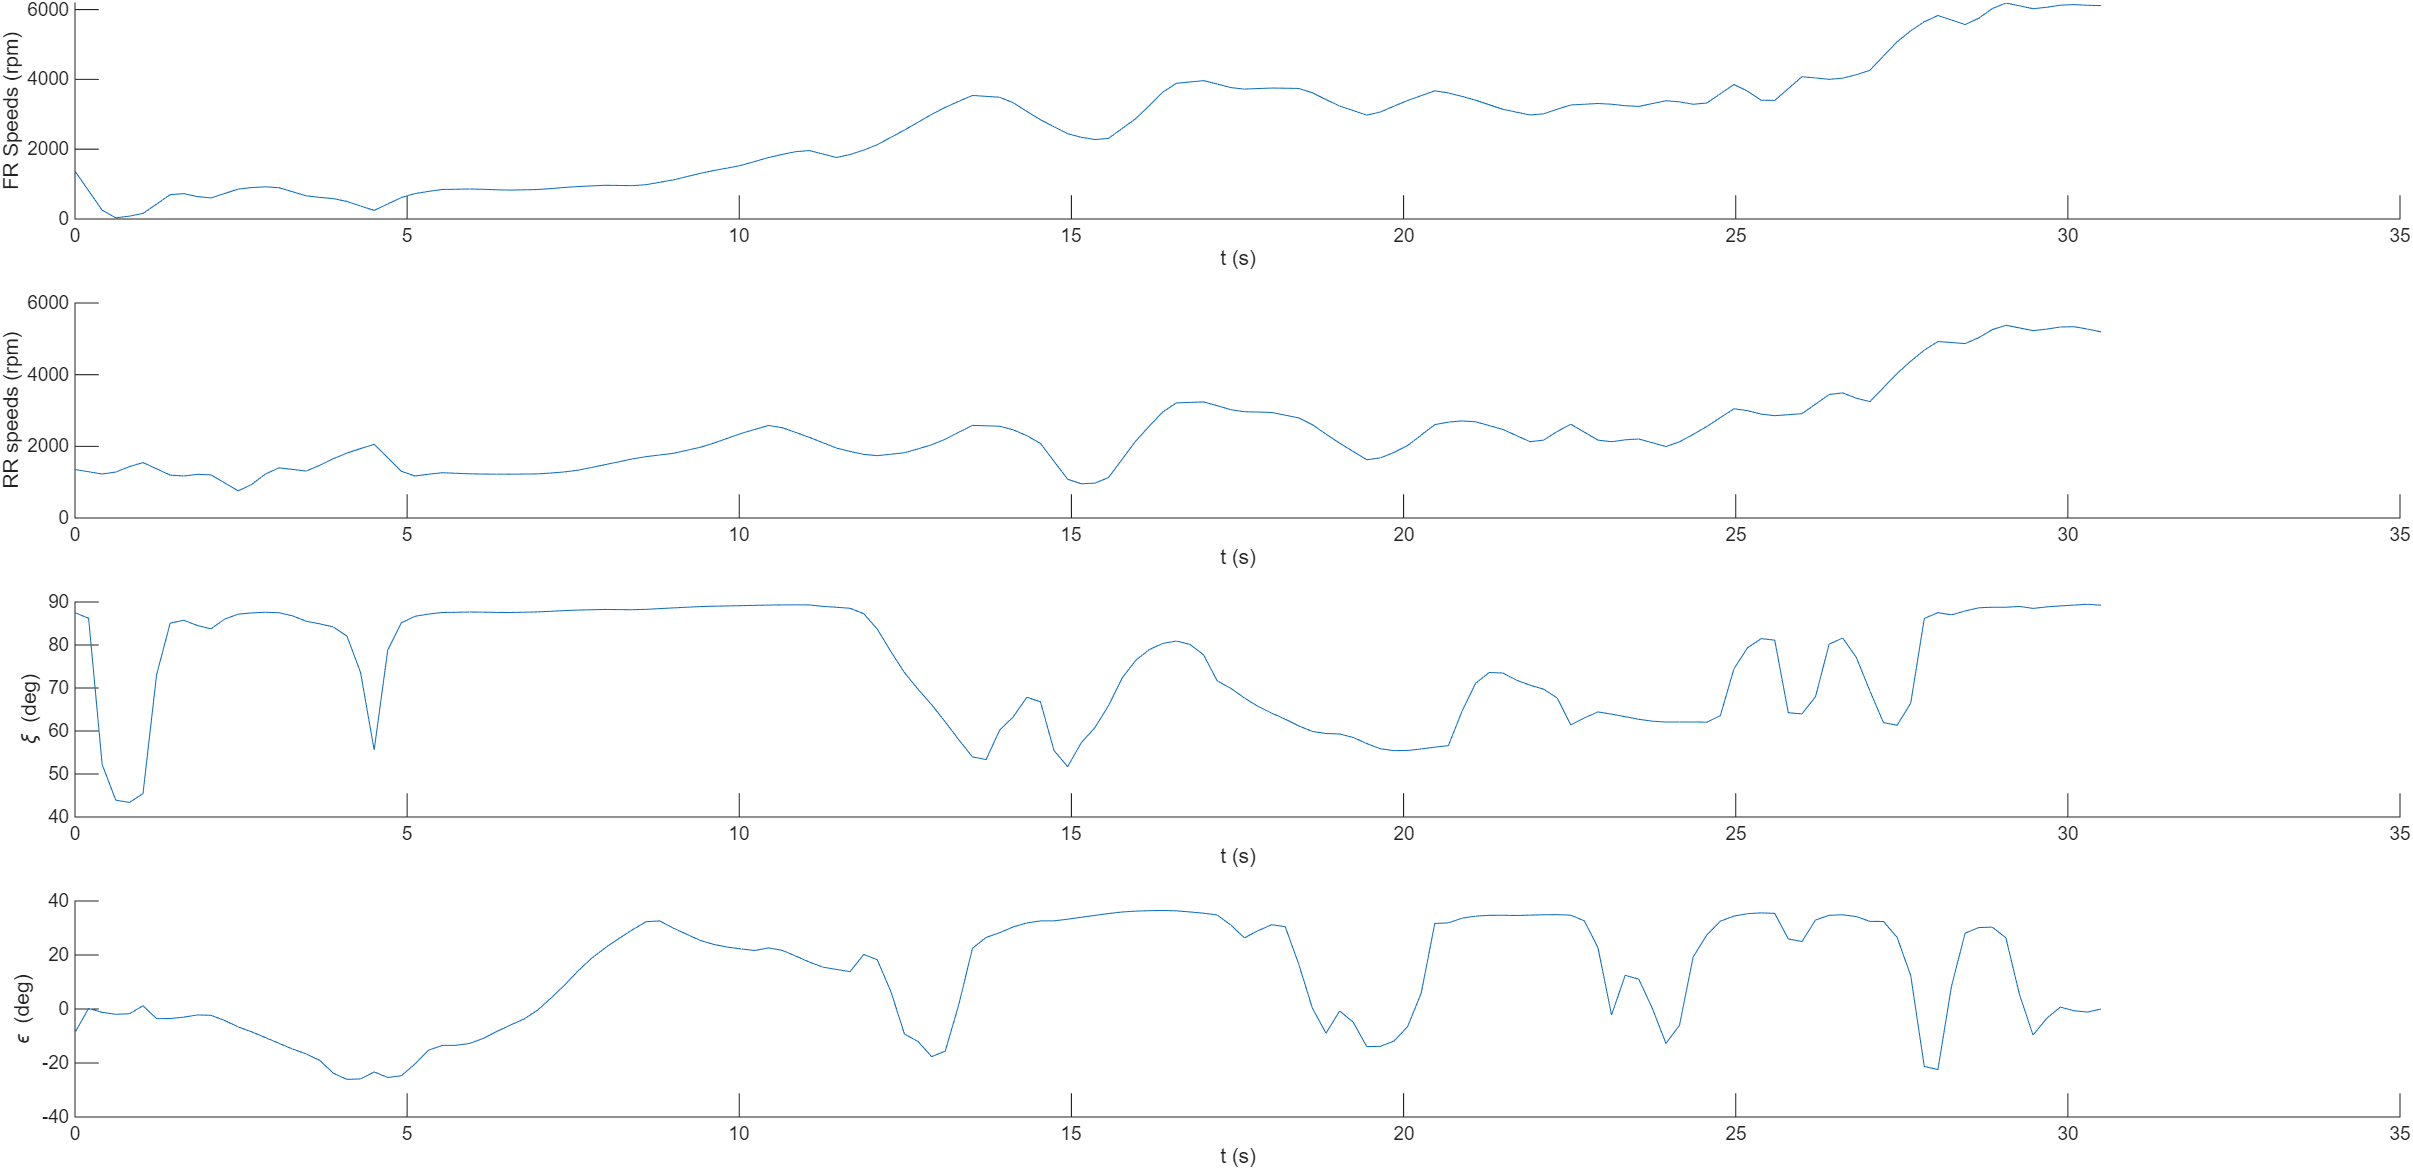
\includegraphics[width=0.8\textwidth]{images/open_loop_control_inputs}
  \caption{Trajectory Optimisation Solution Control Inputs}
  \label{fig:Open-Loop Control}
\end{figure}

\section{Control}
The control of the aircraft is achieved through a time varying linear quadratic regulator (LQR), utilising the optimisation solution as the feedforward term for the longitudinal control and a PID architecture for the lateral stabilisation.

\begin{figure}[htbp]
  \centering
  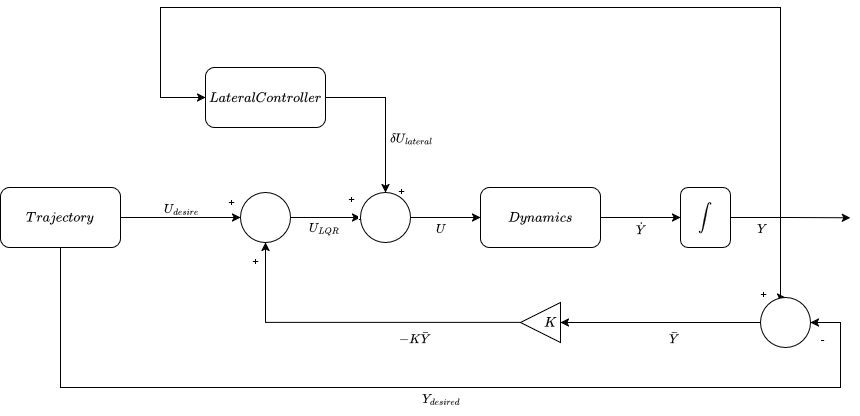
\includegraphics[width=0.8\textwidth]{images/Block Diagram}
  \caption{Longitudinal Control Block Diagram}
  \label{fig:Longitudinal Control Block Diagram}
\end{figure}

The choice of LQR for the longitudinal dynamics was driven by the desire for an efficient control architecture with respect to the goal of this project minimising control energy and to minimise the computation required in real time on the flight controller, as the gains can be precomputed.

\subsection{LQR}
The LQR controller only controls the longitudinal dynamics as shown in section 3.2, therefore $Y_d \in \mathbb{R}^{6 \times \frac{t_f}{\Delta t}}$ and $U_{d} \in \mathbb{R}^{4 \times \frac{t_f}{\Delta t}}$
this is then linearly interpolated to produce $y_{d}(t) \in \mathbb{R}^6$ and $u_{d}(t) \in \mathbb{R}^4$. with these continuous vectors equation \eqref{eq:error_dynamics} can be formed, where $\bar{y}(t)=y(t)-y_{d}(t)$ and $\bar{u}(t)=u(t)-u_{d}(t)$ 
\begin{equation}
\dot{\bar{y}}(t)=f(\bar{y}(t),\bar{u}(t),t) 
\label{eq:error_dynamics}
\end{equation}

As the dynamics of the system are non-linear it was linearised using the Jacobians: $A(t)=\frac{\partial f(t)}{\partial y(t)}$, $B(t)=\frac{\partial f(t)}{\partial u(t)}$ to form equation \eqref{eq:linearised_dynamics}, with a timestep of $1\times 10^{-4}s$



\begin{equation}
\dot{\bar{y}}(t)=A(t)\bar{y}(t)+B(t)\bar{u}(t)
\label{eq:linearised_dynamics}
\end{equation}
\subsubsection{LQR Gains}
The LQR Controller calculates the gains by solving the following cost function:

\begin{equation}
 J_{LQR}=\int_{0}^{\frac{t_{f}}{\Delta t}}  y^{T}(t)Qy(t)+u^{T}(t)Ru(t) \,dt
\label{eq:lqr_cost}
\end{equation}
where $Q \in \mathbb{R}^{6\times6}$ is the state error cost matrix and $R \in \mathbb{R}^{4\times4}$ is the control cost matrix. Both were set using Bryson's rule, stated below.
\begin{equation}
Q_{ii}=\frac{1}{\bar{y}_{i_{max}}^2}, R_{ii}=\frac{1}{\bar{u}_{i_{max}}^2}
\label{eq:brysons_rule}
\end{equation}
resulting in the following values for the Griffin Pro: $Q=diag(4,4,14.5903,1.111\times 10^-3,25,8.2070)$ and $R=diag(4\times 10^{-6},4\times 10^{-6},1.3131\times 10^{4},1.4590\times 10^{3})$. With Q and R selected the differential  Riccati equations can be solved moving back from the terminal point of the trajectory assuming zero final state and input error, to find the gain matrices.

\begin{equation}
-\dot{S}(t)=A^{T}(t)S(t)+S(t)A(t)-S(t)B(t)R^{-1}B^{T}(t)S(t)+Q
\label{eq:riccati}
\end{equation}
\begin{equation}
K(t)=R^{-1}B^{T}(t)S(t)
\label{eq:lqr_gain}
\end{equation}
%https://underactuated.mit.edu/lqr.html

At this point $K \in \mathbb{R}^{4\times6 t_{f} 10000}$ is this much larger than the available memory on most flight controllers and therefore every $10,000^{th}$ term is kept and the rest were discarded forming a new matrix. This is the extent of the precomputation achieved, next  $Y_d\in \mathbb{R}^{6\times t_{f}\Delta t}$, $U_d\in \mathbb{R}^{4\times t_{f}\Delta t}$, and $K_{reduced}\in \mathbb{R}^{4\times 6 t_{f}}$ were imported into the ArduPilot Lua scripting environment.

Within the Lua script the control inputs are converted from their native units (Table 3.1) to $\mu s$ which represents the pulse duration in the aircraft esc. This utilises the ArduPilot function \textit{"SRV\_Channels:setoutput\_pwm\_chan\_timeout"}. The elevator and tilt servos are converted by a linear map, however the motor rpm to $\mu s$ a linear map is employed followed by a SISO PD controller on 

\begin{figure}[htbp]
  \centering
  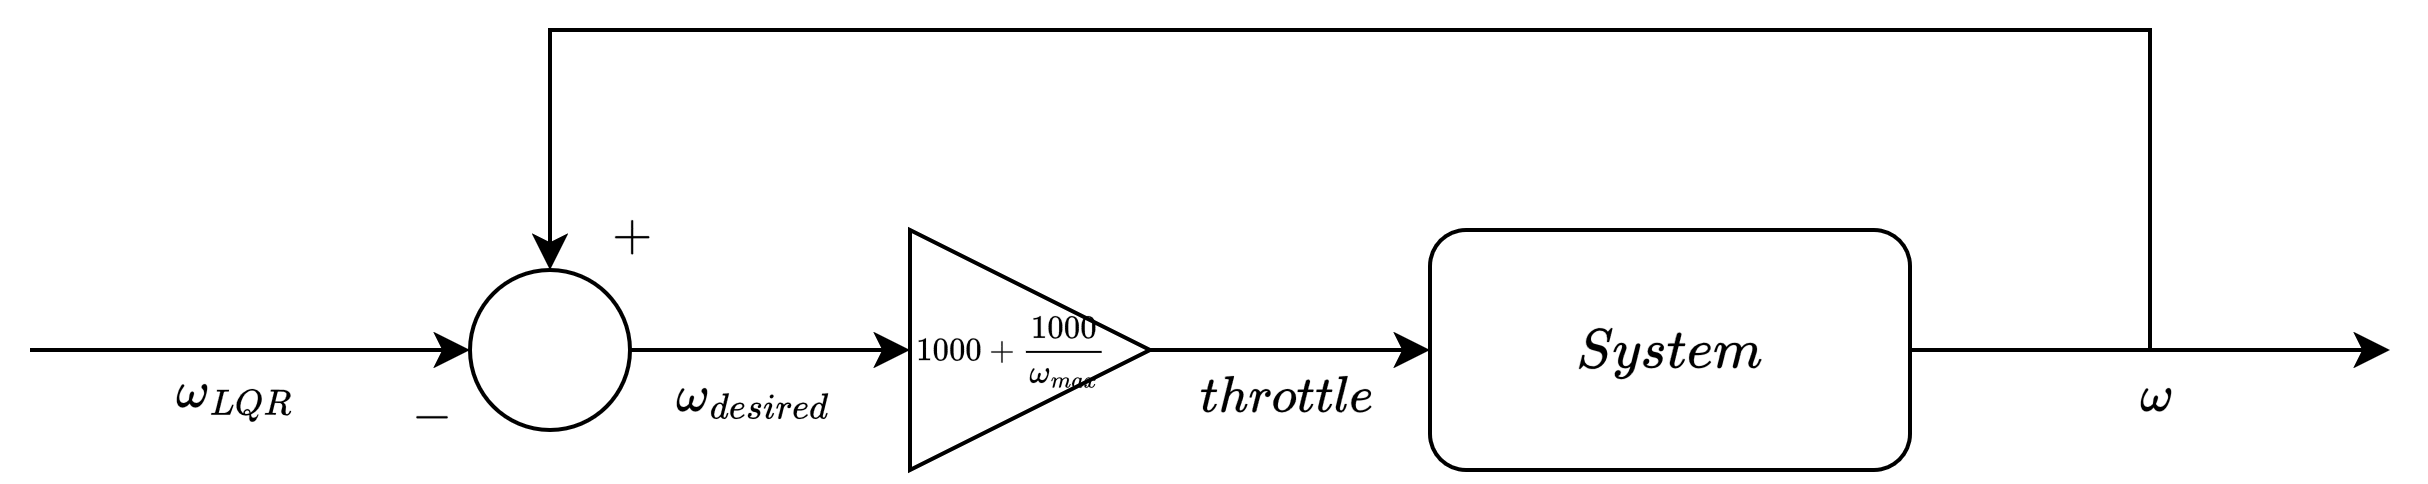
\includegraphics[width=0.8\textwidth]{images/rotor_control}
  \caption{Rotor Control Block Diagram}
  \label{fig:Rotor Control Block Diagram}
\end{figure}




\subsection{Lateral Stabilisation}
As the LQR models is limited to the longitudinal dynamics the lateral stabilisation is a non-optimal series of PD controllers, encompassing roll, yaw, y axis position, controlled through modifiers to the LQR control inputs for the motors and tilt servos, as shown in figure 3.4.

\begin{figure}[htbp]
  \centering
  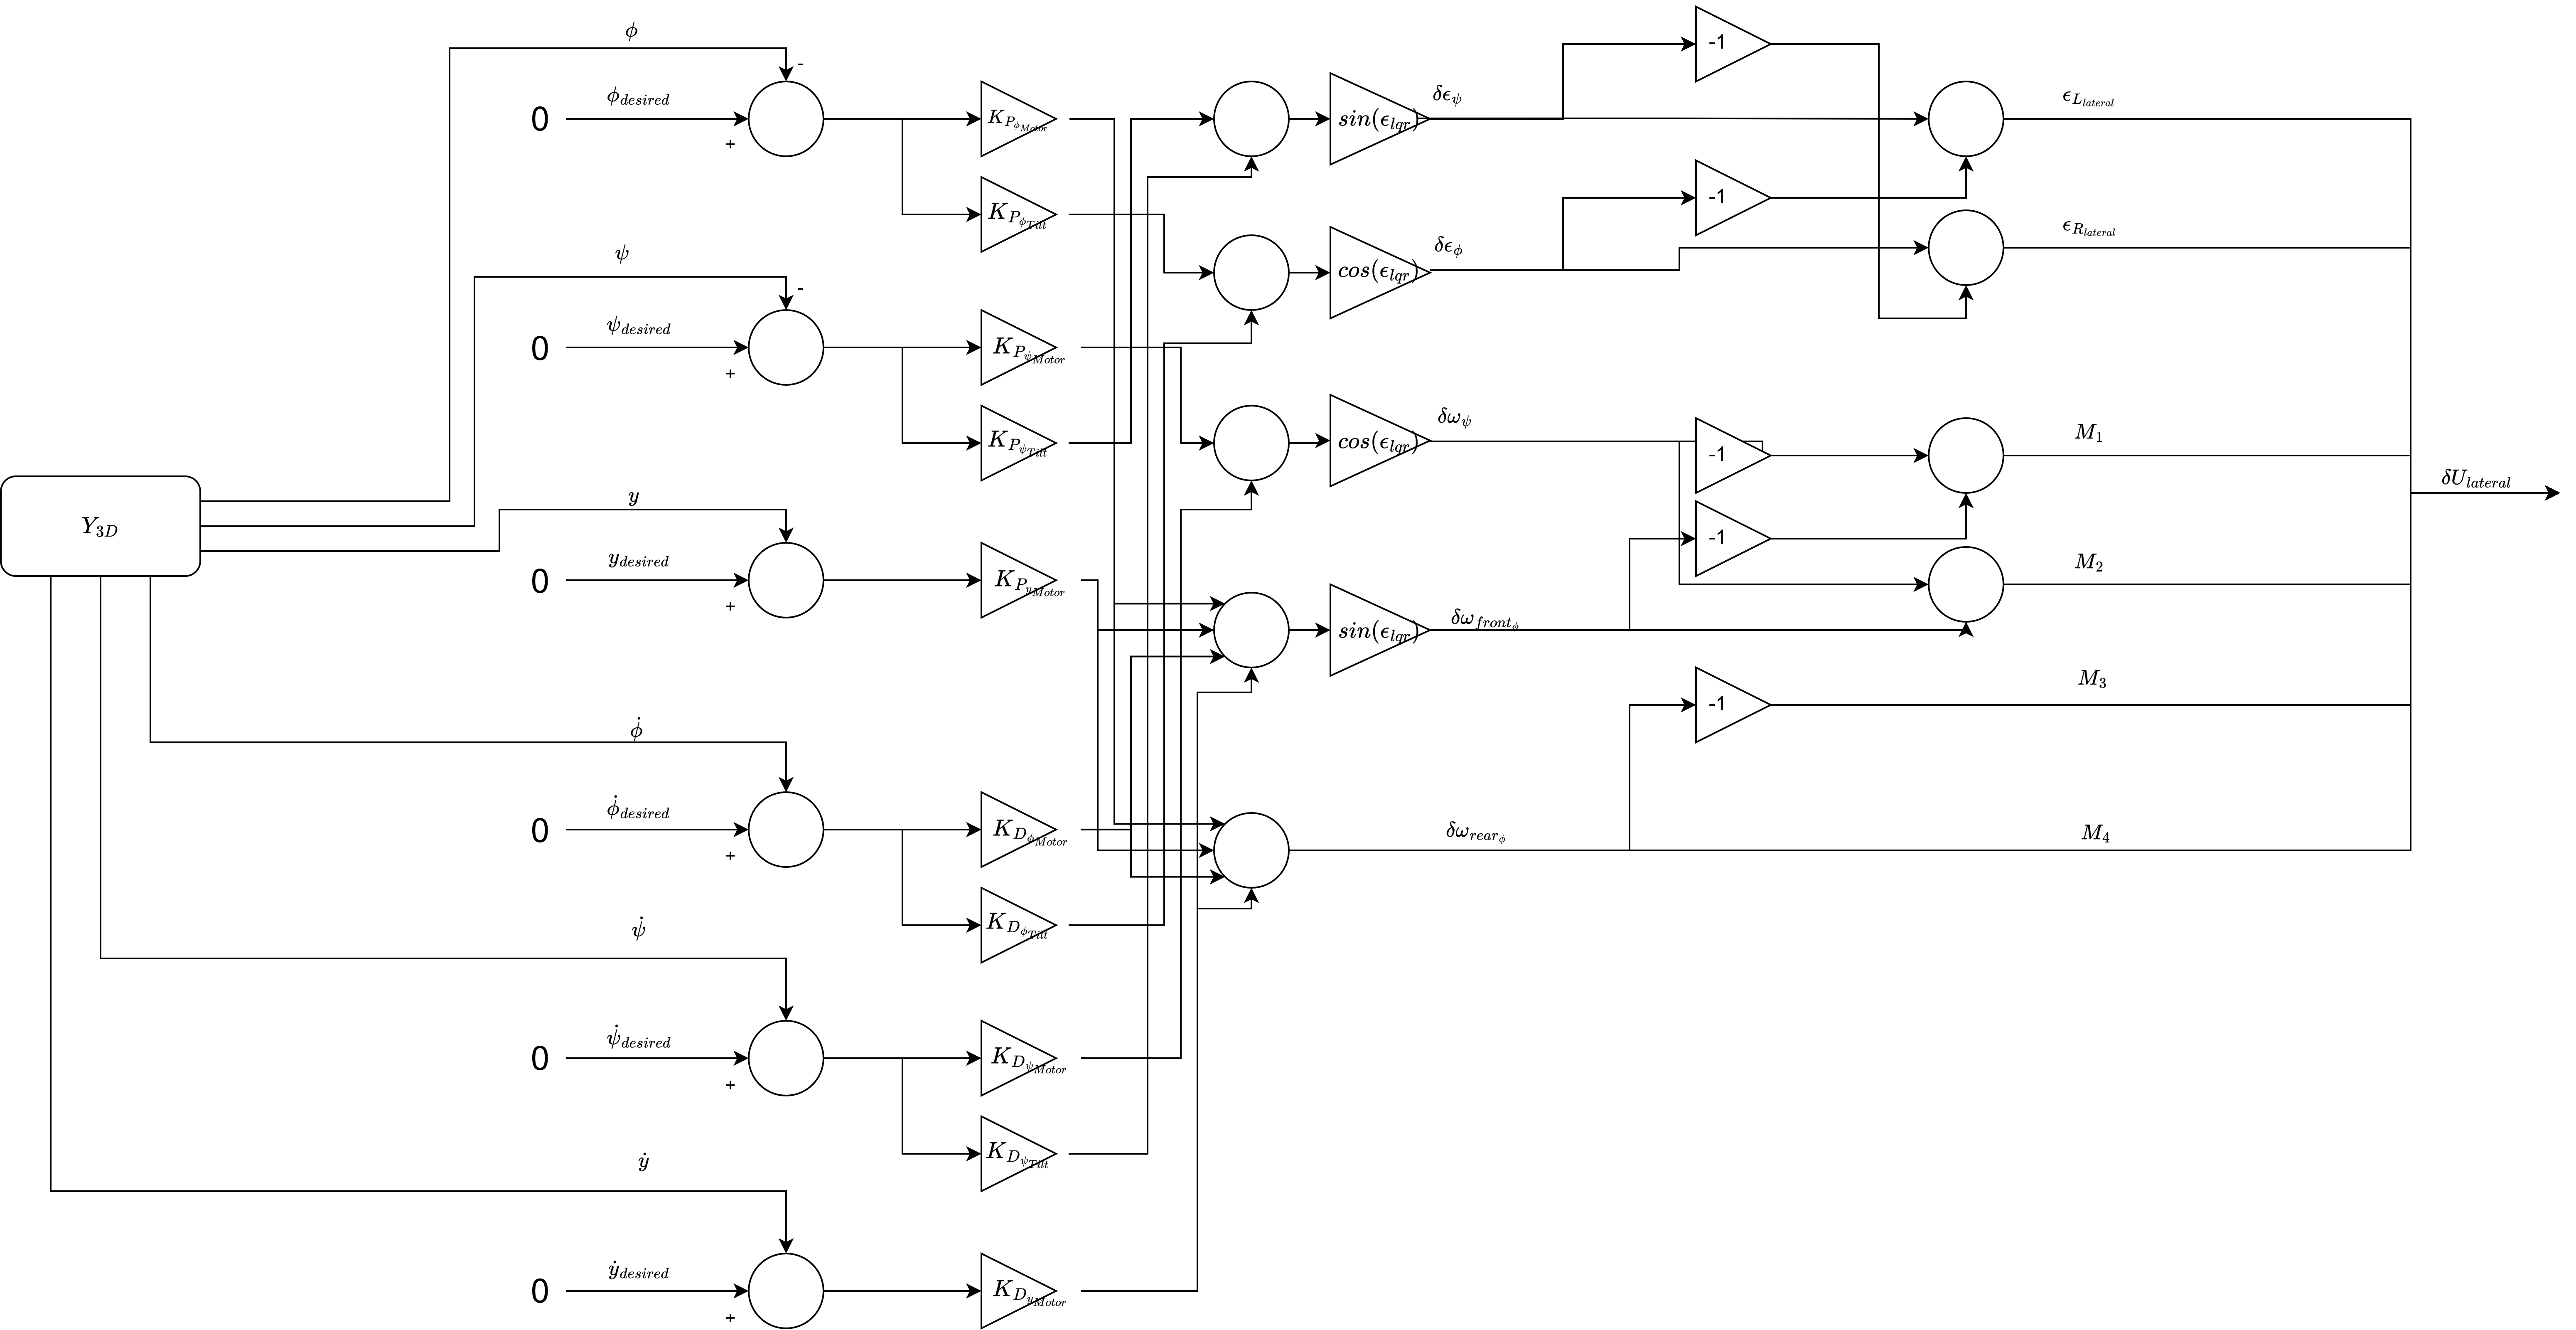
\includegraphics[width=0.8\textwidth]{images/lat_stab}
  \caption{Lateral Control Block Diagram}
  \label{fig:Lateral Control Block Diagram}
\end{figure}

\FloatBarrier
The gains for these PD controllers were tuned with the aid of a large language model agent running simulation in the loop (SITL) runs until the state errors were below the required threshold: $\bar{Y}_{3D}=[0.1745,0.1745,1,0.0524,0.0524,0.5]^{T}|$ resulting in the gains below.
\begin{equation}
a=0.2\Delta t_{lua}+1
\label{eq:gain_scaling}
\end{equation}

\begin{comment}
\begin{table}[ht]
  \centering

  \label{tab:basic_table}
  \begin{tabular}{|l|c|l|c|}
    \hline
    Gain & Value & Gain & Value \\
    \hline
    $K_{P_{\phi_{Motor}}}$ & $\frac{300}{a}$& $K_{D_{\phi_{Motor}}}$ & $\frac{50}{a}$\\
    $K_{P_{\psi_{Motor}}}$ & $\frac{600}{a}$& $K_{D_{\psi_{Motor}}}$ & $\frac{100}{a}$\\
    $K_{P_{y_{Motor}}}$ & $\frac{60}{a}$& $K_{D_{\phi_{Motor}}}$ & $\frac{120}{a}$\\
    $K_{P_{\phi_{\xi}}}$ & $\frac{0.2}{a}$& $K_{D_{\phi_{\xi}}}$ & $\frac{0.03}{a}$\\
    $K_{P_{\phi_{\xi}}}$ & $\frac{0.3}{a}$& $K_{D_{\phi_{\xi}}}$ & $\frac{0.05}{a}$\\
    \hline
  \end{tabular}
  \caption{Lateral Controller Gains}
\end{table}
\end{comment}

\begin{table}[ht]
  \centering

  \label{tab:basic_table}
  \begin{tabular}{|l|c|c|l|c|c|}
    \hline
    Gain & Value & Unit & Gain & Value & Unit\\
    \hline
    $K_{P_{\phi_{Motor}}}$ & $\frac{300}{a}$&$rad->\mu s$& $K_{D_{\phi_{Motor}}}$ & $\frac{50}{a}$&$rad/s->\mu s$\\
    $K_{P_{\psi_{Motor}}}$ & $\frac{600}{a}$&$rad->\mu s$& $K_{D_{\psi_{Motor}}}$ & $\frac{100}{a}$&$rad/s->\mu s$\\
    $K_{P_{y_{Motor}}}$ & $\frac{60}{a}$&$m->\mu s$& $K_{D_{\phi_{Motor}}}$ & $\frac{120}{a}$&$m/s->\mu s$\\
    $K_{P_{\phi_{\xi}}}$ & $\frac{0.2}{a}$&$rad->\mu s$& $K_{D_{\phi_{\xi}}}$ & $\frac{0.03}{a}$&$rad/s->\mu s$\\
    $K_{P_{\phi_{\xi}}}$ & $\frac{0.3}{a}$&$rad->\mu s$& $K_{D_{\phi_{\xi}}}$ & $\frac{0.05}{a}$&$rad/s->\mu s$\\
    \hline
  \end{tabular}
  \caption{Lateral Controller Gains}
\end{table}

where $\Delta t_{lua}$ is the time step between each cycle of the lua script. Each of the five PD controllers is individually clamped, the max tilt alteration is $15\deg$ and $200\mu s$ for the pwm signals.
The layering of the LQR and lateral controllers means that the stability of the system is not guaranteed, as such the poles of the full system were calculated. Figure 3.6 shows the maximum real value of the poles throughout the landing approach.

\begin{figure}[htbp]
  \centering
  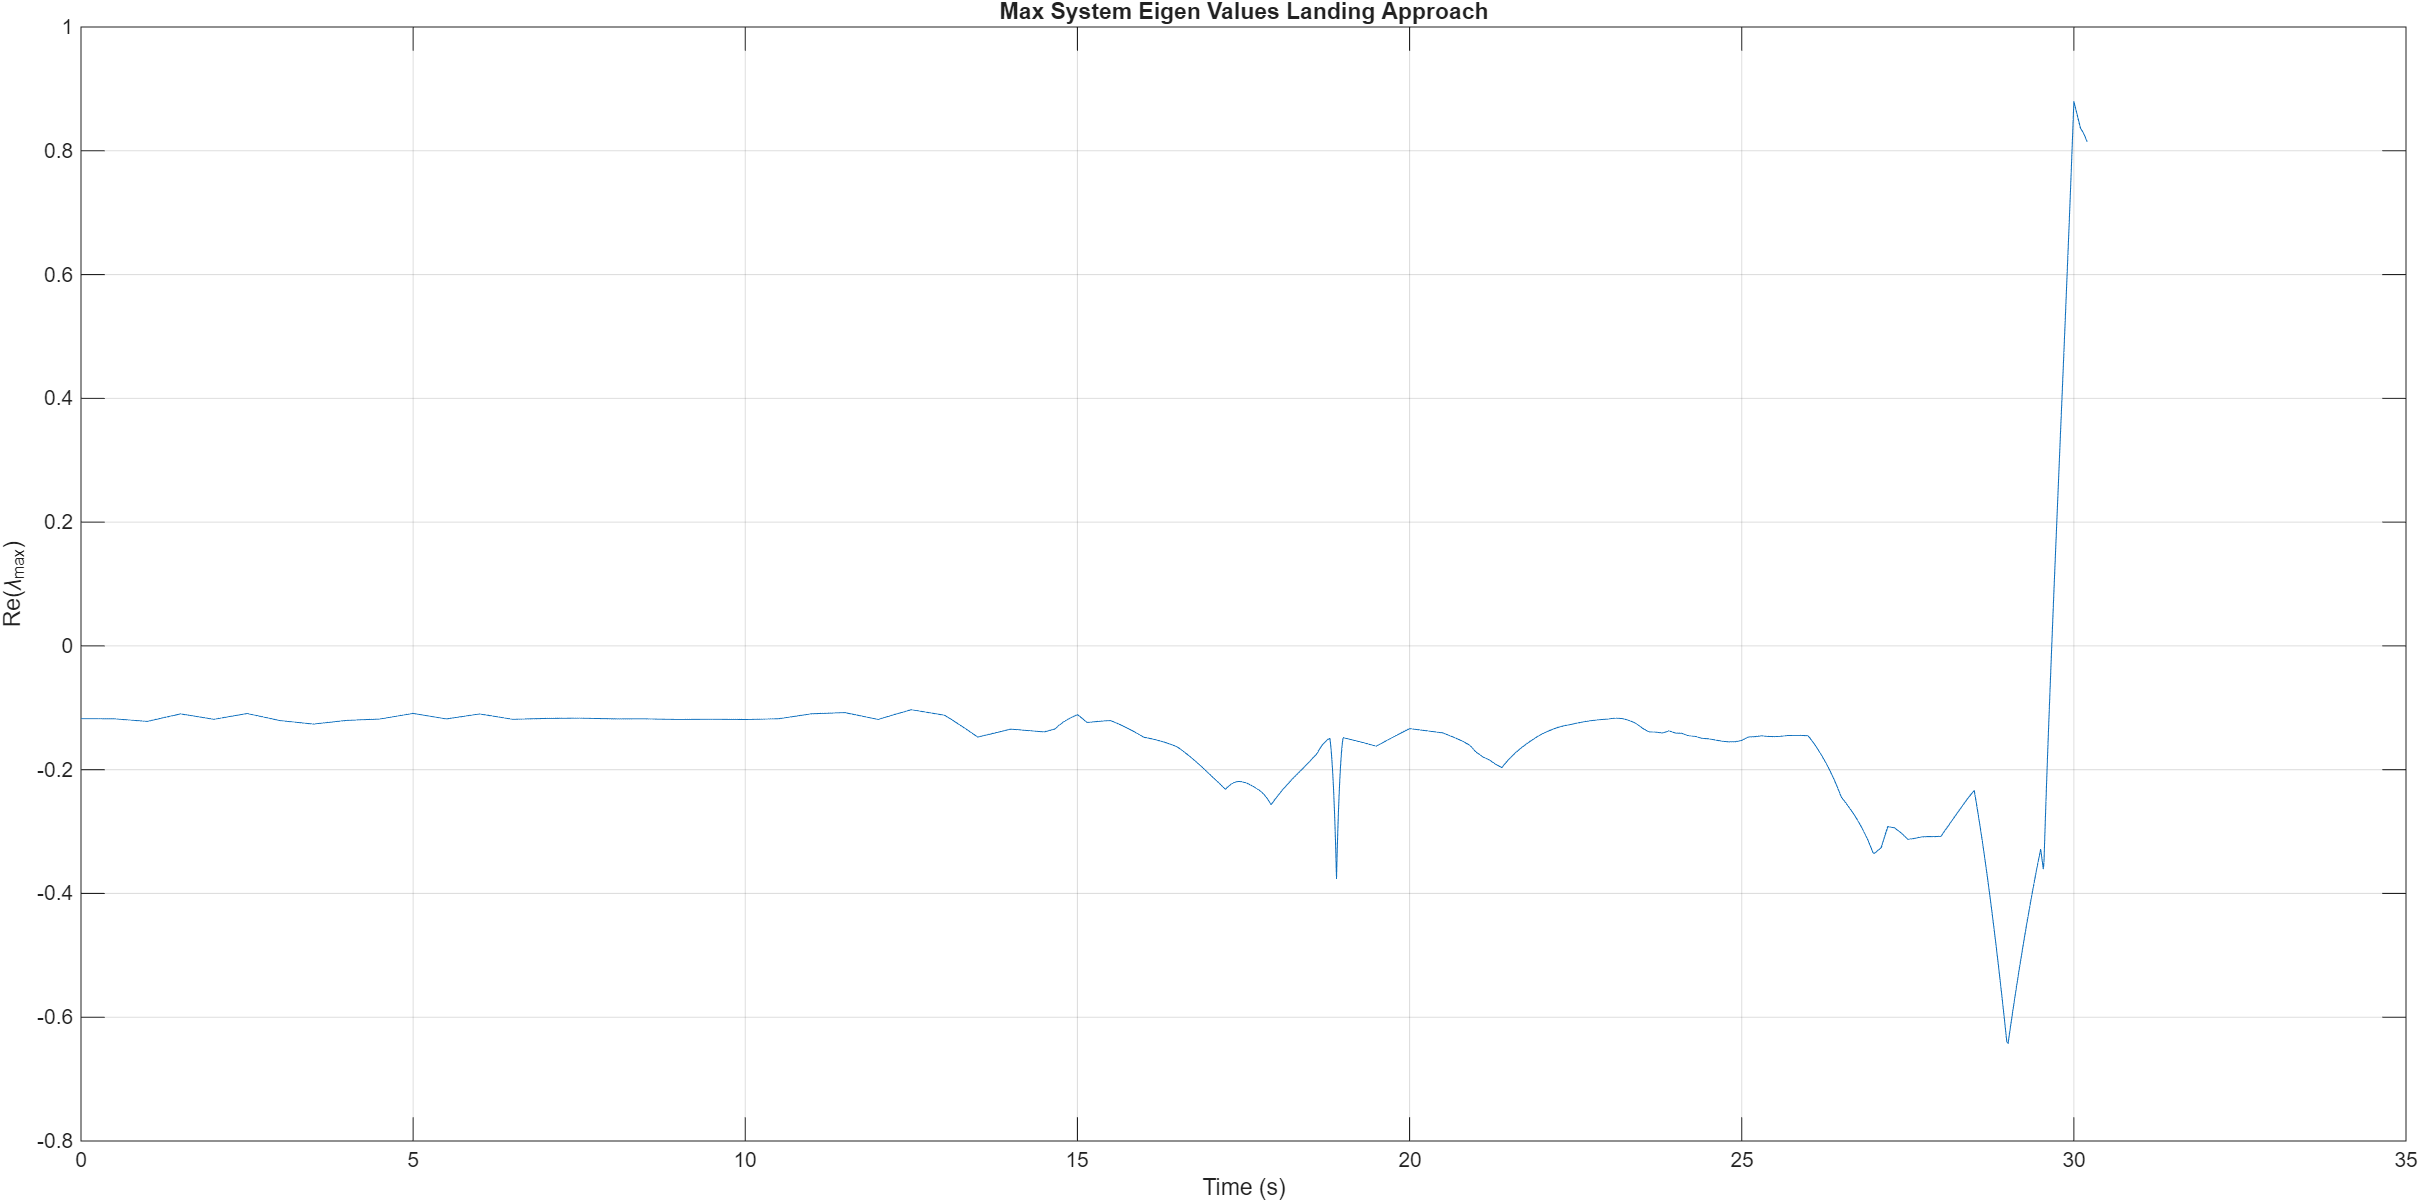
\includegraphics[width=0.8\textwidth]{images/max_real_poles}
  \caption{LQR Re($\lambda_{max}$)}
  \label{fig:lqr rotor poles}
\end{figure}
\FloatBarrier
The max real pole is negative throughout the approach ensuring stability until $t \approx 29.66s$. This is due to the LQR cost function minimising both state error and input cost, meaning that the LQR gains wind-down as the system approaches the time horizon because the error doesn't grow enough before ending to warrant the cost incurred by the rotors.

\begin{figure}[htbp]
  \centering
  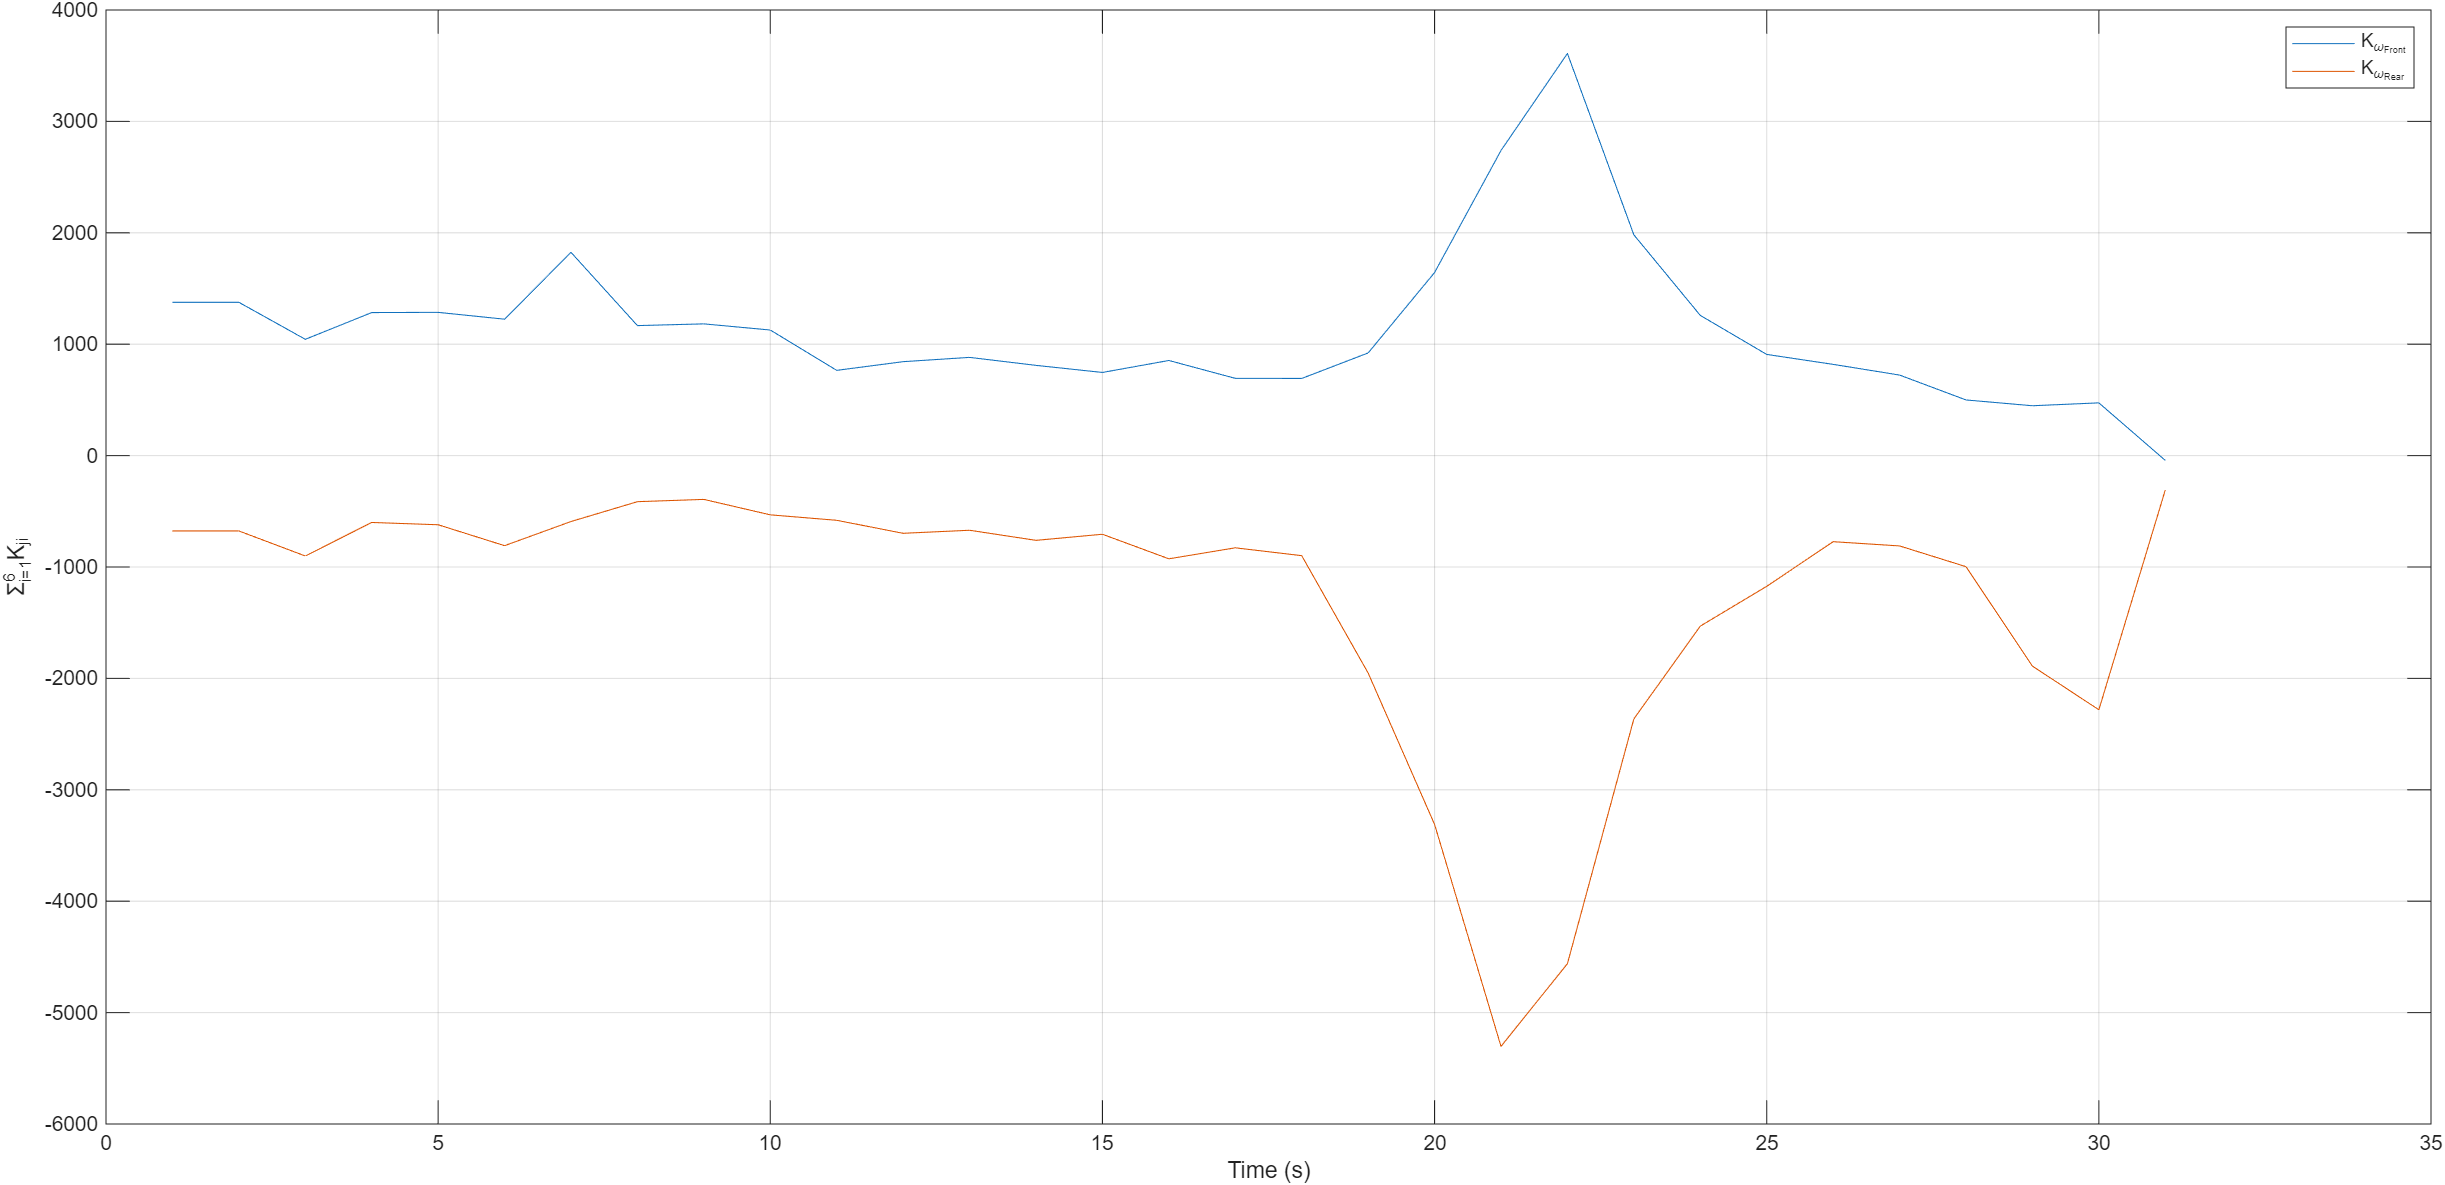
\includegraphics[width=0.8\textwidth]{images/motor_gains}
  \caption{LQR Rotor Gains}
  \label{fig:LQR Rotor Gains}
\end{figure}
\begin{comment}
\begin{figure}[htbp]
  \centering
  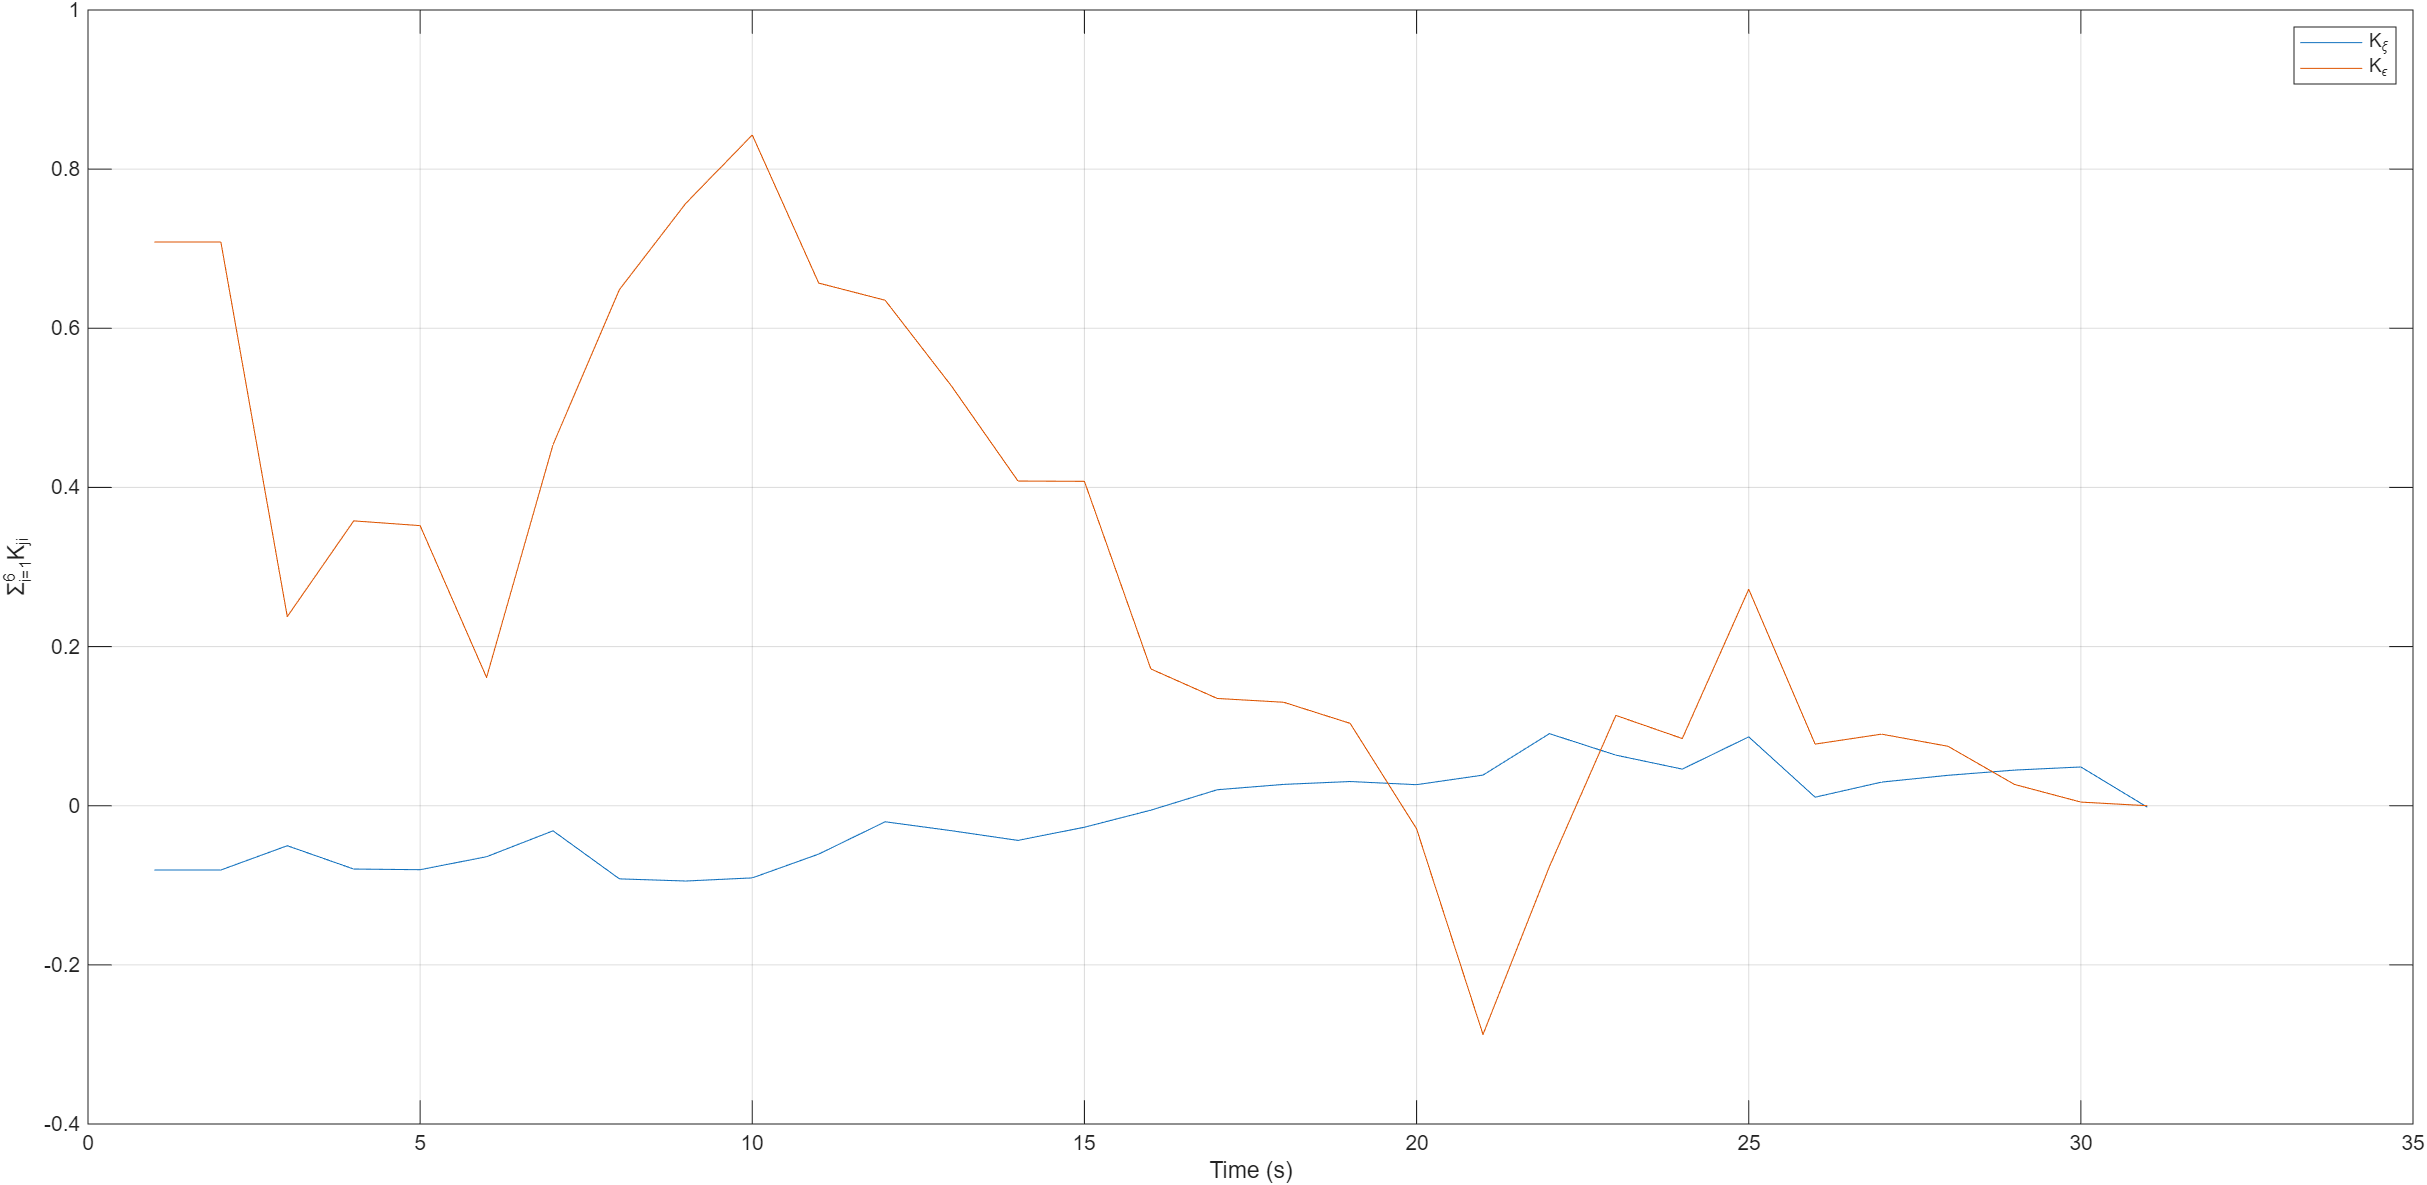
\includegraphics[width=0.8\textwidth]{images/surface_gains}
  \caption{LQR Tilt and Elevator Gains}
  \label{fig:LQR Tilt and Elevator Gains}
\end{figure}
\end{comment}
\FloatBarrier

\begin{comment}
\subsection{Hover}
As part of the vailidation process before moving to real flight tests, a series of hover tests in SITL were conducted, consisting of the aircraft already being in a hover state when Lua controller took over and attempting to hold the hover. The tests included runing lua script at a range of frequencies, and having sudden winds introduced mid hover at different strengths and angles.

\begin{table}[ht]
  \centering

  \label{tab:basic_table}
  \begin{tabular}{|l|c|c|l|c|c|}
    \hline
    Gain & Value & Unit & Gain & Value & Unit\\
    \hline
    $K_{P_{\phi_{Motor}}}$ & $\frac{300}{a}$&$rad->\mu s$& $K_{D_{\phi_{Motor}}}$ & $\frac{50}{a}$&$rad/s->\mu s$\\
    $K_{P_{\psi_{Motor}}}$ & $\frac{600}{a}$&$rad->\mu s$& $K_{D_{\psi_{Motor}}}$ & $\frac{100}{a}$&$rad/s->\mu s$\\
    $K_{P_{y_{Motor}}}$ & $\frac{60}{a}$&$m->\mu s$& $K_{D_{\phi_{Motor}}}$ & $\frac{120}{a}$&$m/s->\mu s$\\
    $K_{P_{\phi_{\xi}}}$ & $\frac{0.2}{a}$&$rad->\mu s$& $K_{D_{\phi_{\xi}}}$ & $\frac{0.03}{a}$&$rad/s->\mu s$\\
    $K_{P_{\phi_{\xi}}}$ & $\frac{0.3}{a}$&$rad->\mu s$& $K_{D_{\phi_{\xi}}}$ & $\frac{0.05}{a}$&$rad/s->\mu s$\\
    \hline
  \end{tabular}
  \caption{Hover Test Results}
\end{table}
\subsection{Level Flight}
\subsection{Landing Approach}
\end{comment}


\section{Simulation Enviroment}
\subsection{Rotor Model}
The public release of ArduPilot's simulation environment doesn't model the non-axial forces of the rotors and therefore I have modified the simulator to model the rotors utilising momentum theory. These changes to the rotor model work with any controller or aircraft running ArduPilot and thus other may wish to use it in their own simulations.
The implementations of these changes follow the same approach as those shown in section 3.1.2, with a varition in how the velocity is the drag term is calculated to work in the three dimenstional simulation.

\begin{equation}
\dot{X}_{front}=R_{IR}(\phi,\theta+\xi-\frac{\pi}{2},\psi), \qquad \dot{X}_{rear}=R_{IR}(\phi,\theta+\xi,\psi), \qquad  {X}=\begin{bmatrix}{x}\\{y}\\{z} \end{bmatrix}
\label{eq:rotor_velocity_sim}
\end{equation}

\section{Safety Features}
\subsection{Altitude Floor}
The Altitude floor is a minimum altitude that if exceeded will cease the control input overrides, returning control to the stock ArduPilot controller. Controller wind up is a concern for the stock controller at handoff, however, from simulation testing it has not been a problem, reference \ref{fig:alt_floor}.

\begin{figure}[htbp]
  \centering
  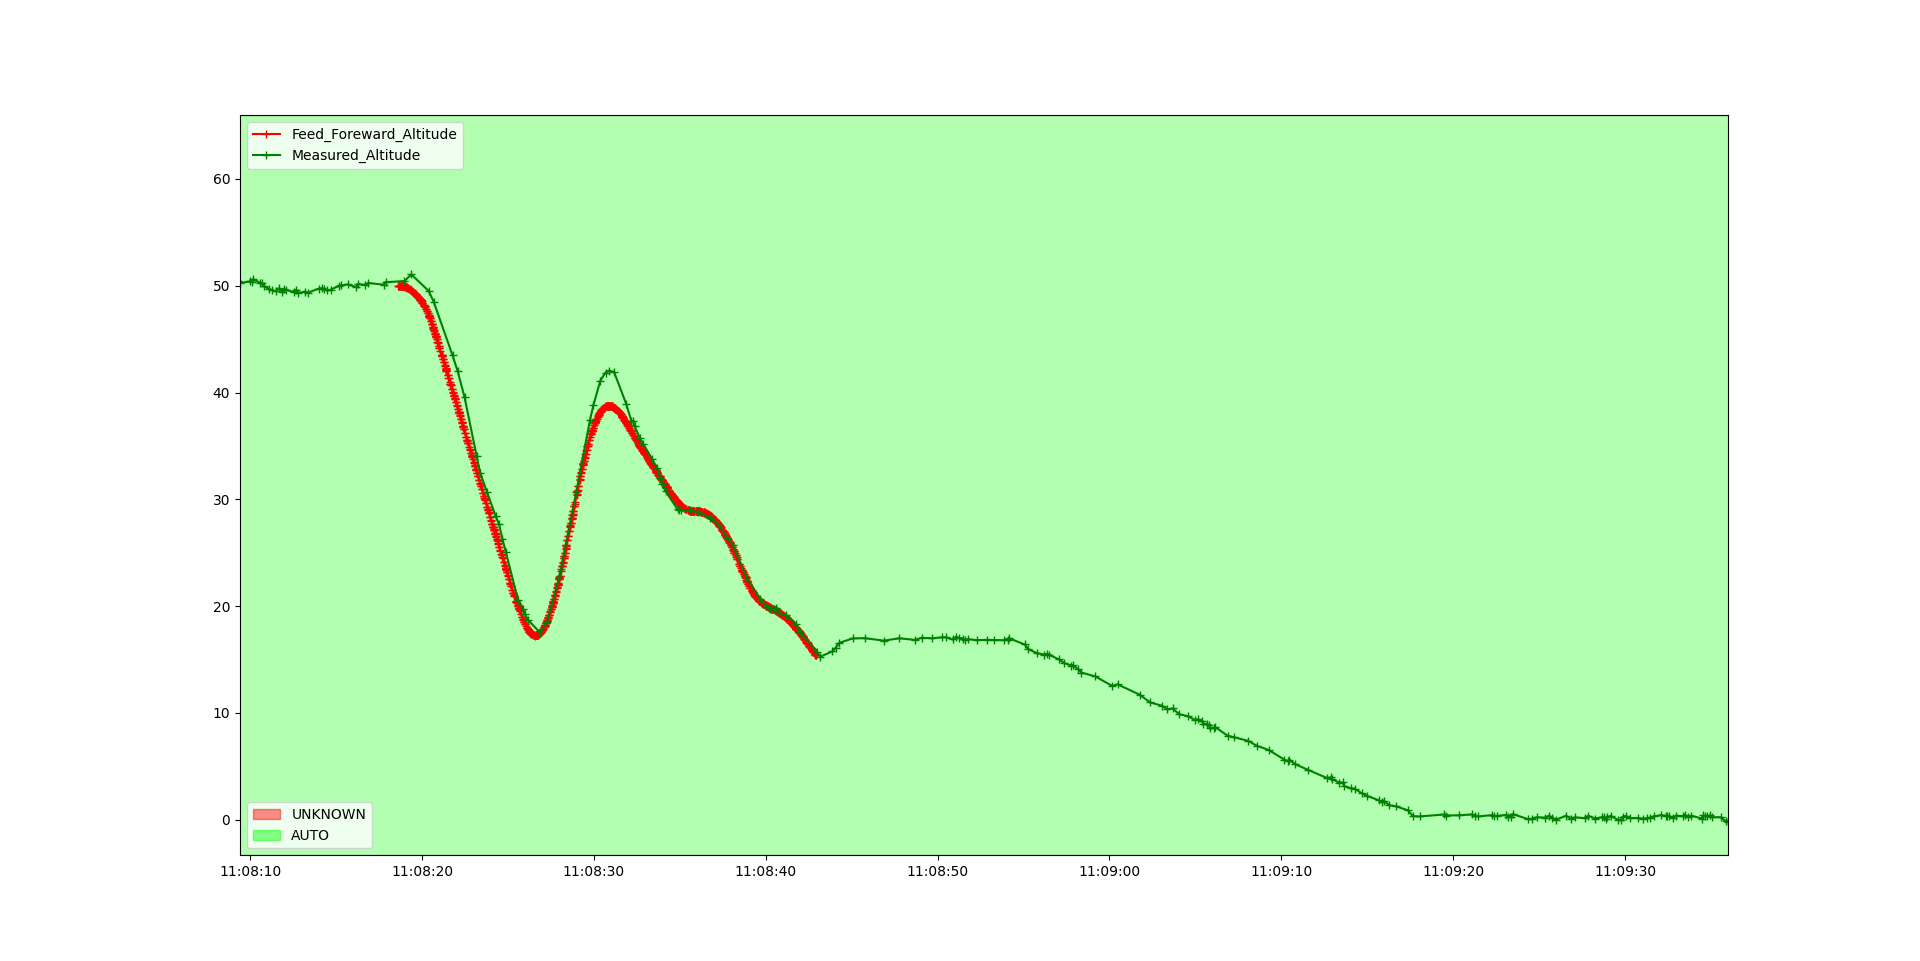
\includegraphics[width=0.8\textwidth]{images/15m_rejection Alt}
  \caption{Altitude Floor Rejected Landing (15m)}
  \label{fig:alt_floor}
\end{figure}

\subsection{State Error Disconnect}
Another method for rejecting the landing sequence is if the norm of the state error surpasses a preset limit. This triggers in two cases, the first is the aircraft failing to track the trajectory (refer to \ref{fig:alt_floor}), the second being a mismatch in the initial condition for example if the trajectory had not been updated and was made for a different altitude approach.

